\label{chap:trab_cor}

Neste capítulo serão apresentados e discutidos os principais trabalhos existentes na literatura que se relacionam com os tópicos que formam a base para o desenvolvimento deste trabalho, com ênfase em: Pré-processamento de Imagem, Segmentação e Detecção de Objetos, Pós-processamento e Reconhecimento de Padrões.

    O projeto proposto visa o desenvolvimento de um sistema embarcado, conectado a uma central para processamento de imagem através de uma rede sem fio. O projeto encontra-se em desenvolvimento, já tendo realizado diversas atividades tais como: revisão da literatura; diagramação das etapas do método proposto; e elaboração de um método para identificação e classificação de imagens. 

     
       %Um dos trabalhos extraídos foi o DeepFish: Accurate underwater live fish recognition with a deep architecture \citeonline{Qin:2016},  que propõe um framework no reconhecimento de objetos dentro d’água, esse trabalho foi fundamental para seleção de um método para identificação de imagens utilizando redes neurais convolutivas.

       Visando documentar o fluxo de execução do método proposto neste trabalho, foi realizado a diagramação do método proposto, utilizando diagramas da UML e caixas, com a especificação de tecnologias como linguagens de programação e métodos encontrados na literatura a serem utilizadas no projeto do sistema computacional proposto neste trabalho. Logo, o sistema proposto é apresentado como um sistema embarcado usando  microcontroladores (neste caso, neste projeto esta sendo testado as plataformas Arduino e Raspberry Pi), sensores óticos, etc. 

       O sistema embarcado proposto será baseado em detecção via um sensor de captura ótica, que ficará submerso em água, acoplados à uma boia, que terá um conexão sem fio com um celular ou computador. O pré-processamento da imagem é feito com diversos filtros e processos para correção de anomalias na imagem.

       O módulo  de detecção de objetos do sistema proposto, ainda em desenvolvimento, está sendo aperfeiçoado para interagir de forma inteligente com o ambiente observado, isso significa que filtros serão automaticamente aplicados para melhorar a detecção de objetos em ambiente com pouca iluminação e com alta turbidez. Com base na estrutura do sistema computacional proposto, ainda identificamos alguns desafios a serem superados para a conclusão do trabalho proposto, tais como: a integração dos diferentes módulos (exemplo, detecção de objetos) em um único sistema; consumo  energético; estrutura e prototipação dos sistema em ambientes reais como rios. 
	

 

%\section{Análise e publicação de resultados}
%A Tabela detalha os resultados gerais de publicações identificadas pela máquina de busca, bem como o número de publicações aceitas em cada um dos filtros executados, de acordo com a expressão de busca executada na biblioteca Scopus. \textcolor{red}{adicionar tabela de resultados.}


\section{Análise dos trabalhos correlatos}
Nesta seção serão serão feitas análises dos trabalhos correlatos, mostrando as diferenças entre o projeto proposto e os trabalhos encontrados, como tecnologias e estruturas utilizads.

\subsection{DeepFish: Accurate underwater live fish recognition with deep architecture}
Um \textit{framework} baseado em uma \textit{Convolutional Neural Network} foi proposto por \citeonline{Qin:2016} para reconhecimento de peixes em vídeos gravados submersos em água. No trabalho as imagens de fundo são removidas utilizando métodos baseados em decomposição de matrizes esparsas e de baixo nível, removendo assim apenas o fundo da imagem, deixando somente o peixe.

Os dados extraídos são passados para camadas de convolução depois para uma camada não linear, em seguida é feita a classificação utilizando SVM (Support Vector Machine). A taxa de aprendizado diminui a medida que a quantidade de parâmetros são adicionados, necessitando assim de uma otimização no filtro de aprendizado. 

O método do trabalho de \citeonline{Qin2016}, pode ser visto na \autoref{fig:trainignqin}, onde os passos do \textit{framework} são mostrados. Onde os filtros são escolhidos, as imagens processadas pela rede neural profunda e processos para extração de atributos, após essas etapas a saída final alimenta uma máquina de vetor de suporte linear.
\begin{figure}[h]
	\caption{\label{fig:trainignqin}\textit{Pipeline} do \textit{framework} proposto.}
	\begin{center}
	    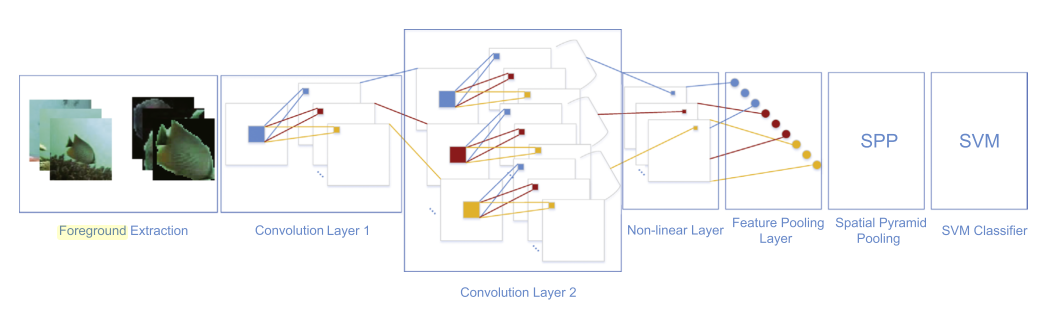
\includegraphics[width=1\textwidth]{resources/trainingqin}
	\end{center}
	\legend{Fonte: \cite{Qin:2016}}
\end{figure}
   

Similar ao trabalho de \citeonline{Qin:2016}, o método apresentado nesse trabalho de conclusão de curso propõe um método para detecção, porém não à identificação de imagens. A classificação será feita utilizando métodos baseados em \textit{Convolutional Neural Network} assim como no trabalho de \citeonline{Qin:2016}.

%Com o \textit{framework} proposto pelo trabalho espera-se avanços na área de pesquisas sobre reconhecimento de peixes, explorar soluções no reconhecimento de objetos submersos. Beneficiar biológos, ecologistas e fins comerciais como fazendas de peixes.


\subsection{A Feature Learning and Object Recognition Framework for Underwater Fish Images}
\citeonline{Chuang2016AImages} propõe um \textit{framework} para reconhecimento de peixes em baixo d'água, que consiste em uma técnica de de aprendizagem totalmente não supervisionada e um classificador resistente a erros. Os dados são iniciados com base em algumas características, depois passados por alguns critérios de separação. 

O classificador, tem uma abordagem não supervisionada que gera uma classe de hierarquia binária, onde cada nó é um classificador. Os experimentos mostram que o \textit{framework} proposto é preciso tanto em situações onde a base de dados é públicas quanto em ambientes controlados com alta incerteza.

\begin{figure}[h]
	\caption{\label{fig:trainingchuan}Proposta de treinamento não supervisionada .}
	\begin{center}
	    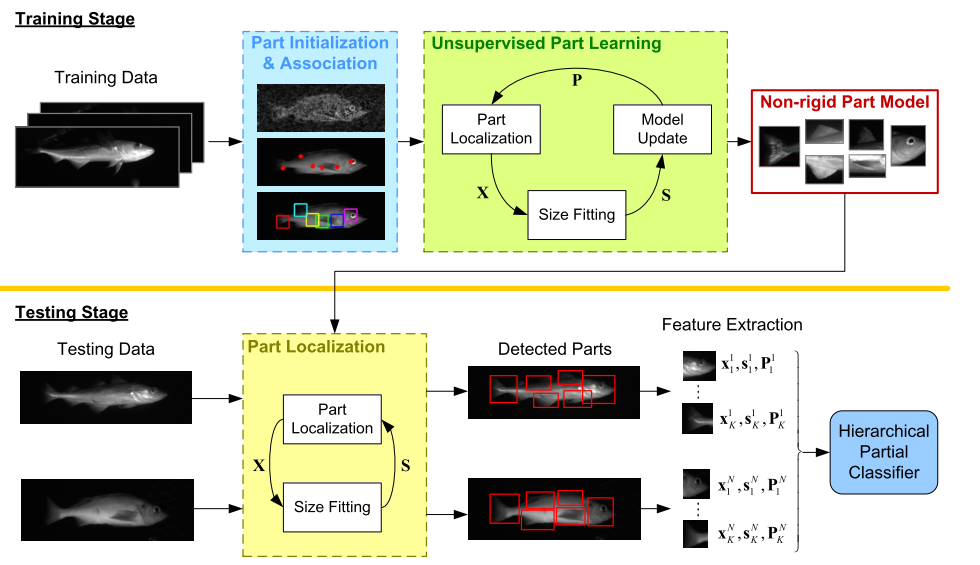
\includegraphics[width=0.9\textwidth]{resources/training}
	\end{center}
	\legend{Fonte: \cite{Chuang2016AImages}}
\end{figure}
   

A utilização do trabalho de \citeonline{Chuang2016AImages} como referência irá auxilar em uma abordagem de aprendizado resistente a erros, que irá auxiliar na confiabilidade de informação, uma vez que o sistema proposto no trabalho irá auxilar mergulhadores em lugares de riscos, em águas com alta turbidez. 


\subsection{A Vision Based System for Object Detection in Underwater Images.}

O trabalho de \citeonline{FORESTI2000AImages} propõe um sistema como mostra o fluxograma na ~\ref{fig:forestflow} (veículo autônomo) para detecção e rastreio de objetos submersos em água, o sistema faz detecção automática de canos (que podem se estender por quilômetros) e posicionamento autônomo baseado nas detecções.

São aplicados alguns filtros para compensação de cor e dimensionamento na imagem. Depois do dimensionamento essas imagens ganham tamanhos de 1/16 para detecção de bordas (para encontrar canos) e 1/32 para encontrar anodos em canos.
\begin{figure}[h]
	\caption{\label{fig:forestflow}Proposta do sistema.}
	\begin{center}
	    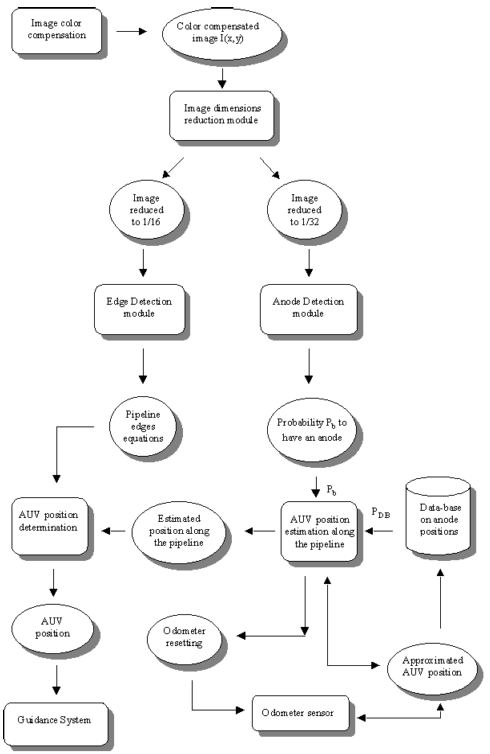
\includegraphics[width=0.5\textwidth]{resources/flowchartforest}
	\end{center}
	\legend{Fonte: \cite{FORESTI2000AImages}}
\end{figure}

A identificação dos objetos é feita utilizando redes neurais, que classificando a imagem em tempo real, verificando se há obstáculos. Essas informações auxiliam na navegação automática do veículo, traçando rotas e caminhos através das imagens processadas e ressonância geométrica.

O sistema proposto por \citeonline{Gentili2000A.} consegue detectar canos e outras estruturas, mesmo com os problemas causados pela falta de luminosidade, dispersão e atenuação da luz e problemas como areia e detritos sobre canos.

Comparado ao trabalho que está sendo desenvolvido, um sistema irá trabalhar na detecção de objetos, e estipulação do tamanho desses objetos, afim de avisar os possíveis perigos que se escondem de baixo d'água.

\subsection{Automatic Plankton Image Recognition}

O trabalho de \citeonline{tang1998automatic} propõe um sistema que utiliza redes neurais para classificação de  padrões para identificar um grande número de imagens de plânctons, detectadas em tempo real por um sistema de microscópio de vídeo subaquático rebocado. O sistema que utiliza características granulométricas em escala de cinza como um poderoso descritor de padrão que captura as assinaturas de forma e textura, capaz de detectar automaticamente plânctons, auxiliando no rastreio da proliferação da vida marinha que se alimentam de plânctons e entender o complexo ecossistema marinho.

flow\begin{figure}[h]
	\caption{\label{fig:tangnet} Quantização vetorial de aprendizado da rede neural.}
	\begin{center}
	    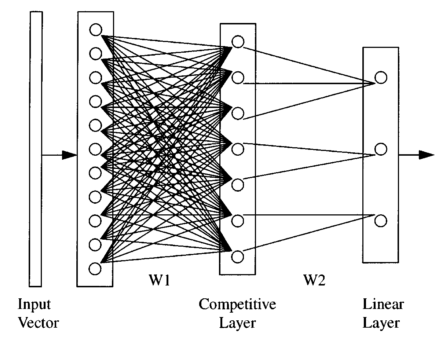
\includegraphics[width=0.5\textwidth]{resources/neuralnet}
	\end{center}
	\legend{Fonte: \cite{tang1998automatic}}
\end{figure}

No trabalho \citeonline{tang1998automatic} o sistema proposto é capaz de identificar plânctons para compreensão de como o ecossistema marinho funciona. Em comparação, o método apresentado neste trabalho de conclusão de curso é proposto um método para detecção, porém não à identificação de objetos em ambiente aquático submersos em águas turvas, mas sim uma classificação de que tipo de objeto e uma especulação do seu tamanho. A classificação será feita utilizando métodos baseados em \textit{Convolutional Neural Network}, utilizando o \textit{framework} \textbf{Tensorflow}.

\section{Automatic underwater image pre-processing}
Esse trabalho propõe um filtro de processamento para restauração de imagens de ambiente submersos. Pela da transmissão de propriedades da luz sobre a água. Imagens de ambiente submersos sofrem pela perda de distância na captura, distorção de luz, baixo contraste, baixa saturação de cor e outros problemas. Os métodos de processamento de imagens atuais focam em distorção e atenuação causados pela luz e precisam de conhecimento do ambiente que está sendo estudado. O algoritmo proposto pelo trabalho de \cite{bazeille2006}, é um algoritmo que automatiza o pré-processamento de imagens submersas.  a filtro reduz as pertubações nas imagens submersas, e melhorando a qualidade da imagem.



%Processos independentes e sucessivos que corrigem a ilumação não uniforme, supressão de ruídos, melhoria no contraste e ajuste de cor, aplicados com base na detecção de bordas.
%\section{Foreground Extraction of underwater Videos via Sparse and Low-rank Matrix Decomposition}


%\section{Análise dos trabalhos correlatos}
%Nessa sessão será abordado as características similares e comparações dos trabalhos correlatos com o desenvolvimento do trabalho de conclusão de curso. Mostrando as técnicas e métodos utilizados.

%\subsection{Pré-processamento}
%O pré-processamento da imagem é um passo fundamental para poupar processamento, uma vez que será menos dados a serem processados, diminuindo tempo e gastos energéticos, e como o trabalho a ser desenvolvido será um sistema embarcado, o aperfeiçoamento e eficiência são peças fundamentais.

%No trabalho de \citeonline{Qin:2016}, as imagens de fundo são removidas utilizando métodos baseados em decomposição de matrizes esparsas e de baixo nível, removendo assim apenas o fundo da imagem, deixando somente o peixe.

%Já no trabalho de \citeonline{FORESTI2000AImages}, são aplicados alguns filtros para compensação de cor e dimensionamento na imagem. Depois do dimensionamento essas imagens ganham tamanhos de 1/16 para detecção de bordas (para encontrar canos) e 1/32 para encontrar anodos em canos.

%No trabalho de \citeonline{Chuang2016AImages} um filtro Gaussiano é aplicado junto uma transformada de Fourier para estimar a saliência na imagem, em seguida uma máscara é utilizada para descartar pontos no plano de fundo da imagem. em seguida a extração do fundo é feita por técnicas como \textit{GrabCut Segmentation}.

%\begin{itemize}
%\item Reconhecimento de objetos (OR): Algum objeto ou ser vivo foi reconhecido.
%\item Turbidez no ambiente (TA): O ambiente estudado tinha baixa visibilidade e/ou algum tipo de detrito ou interferência .
%\item Sistema desenvolvido para captura de imagens submersas (SC): Algum sistema criado para capturar imagens submersas foi desenvolvido.
%\item Foco em baixo custo (BC): O projeto foi desenvolvido com ideia de baixo custo ou eficiência energética. 
%\end{itemize}


%\begin{table}[H]
%\caption{Comparações}
%\small
%\centering
%\begin{tabular}{|p{8cm}|c | c | c | c |}
 
%	\hline \textbf{Trabalhos} & \textbf{OR} & \textbf{TA} & \textbf{SC} & \textbf{BC}\\ \hline
	
 %   Computer Vision for ocean observing & X & X &  &  \\ \hline
	
  %  DeepFish: Accurate underwater live fish recognition with deep architecture & \centering X & X &  & X \\ \hline
      
  %    A Vision Based System for Object Detection in Underwater Images & X & X & & X  \\ \hline  
      
   %     Automatic underwater image pre-processing &  & X & &   \\ \hline
        
        
    %    A Feature Learning and Object Recognition Framework for Underwater Fish Images &  & X & &   \\ \hline
	%\end{tabular}

%\end{table}

